\section{序論}\label{ux5e8fux8ad6}

\subsection{背景}\label{ux80ccux666f}

\subsubsection{チューリングテスト}\label{ux30c1ux30e5ux30fcux30eaux30f3ux30b0ux30c6ux30b9ux30c8}

\subsubsection{IoTの普及}\label{iotux306eux666eux53ca}

\subsection{目的}\label{ux76eeux7684}

\subsection{本論文の構成}\label{ux672cux8ad6ux6587ux306eux69cbux6210}

\section{研究領域の背景}\label{ux7814ux7a76ux9818ux57dfux306eux80ccux666f}

\subsection{問題提起}\label{ux554fux984cux63d0ux8d77}

\subsection{関連研究}\label{ux95a2ux9023ux7814ux7a76}

\section{Physical Certification}\label{physical-certification}

\subsection{概要}\label{ux6982ux8981}

\subsection{目的}\label{ux76eeux7684-1}

\subsection{特徴}\label{ux7279ux5fb4}

\subsection{提案システムの利用例}\label{ux63d0ux6848ux30b7ux30b9ux30c6ux30e0ux306eux5229ux7528ux4f8b}

\subsection{手法}\label{ux624bux6cd5}

\subsubsection{システム構成}\label{ux30b7ux30b9ux30c6ux30e0ux69cbux6210}

本システムは出題するタスクを表示する「Webブラウザ」,日常生活で発生するタスクを記録,
Webブラウザに対してタスクの内容を送信する「IoTサーバ」,
日常タスクを感知しIoTサーバに送信する「センサ群」の3つのシステムで構成されている.

\subsubsection{Webブラウザ}\label{webux30d6ux30e9ux30a6ux30b6}

Webブラウザの主な役割はユーザに対してタスクを表示し遂行を促すことと,
完了の通知を受取り, ユーザのWebサービスの利用を許可することである.
ユーザがWebサービス利用でチューリングテストを行うとWebブラウザからIoTサーバに対して発生しているタスクを要求する.
WebブラウザはIoTサーバからタスクを受け取るとタスクの詳細をユーザに表示し,
タスクの遂行を促す.
タスクの完了の通知をIoTサーバから受け取ることでユーザにWebサービスの利用を許可する.
IoTサーバの主な役割はセンサー群から日常生活のタスクの発生や完了状況をデータベースに記録とWebブラウザに対して遂行させるタスクとタスク完了の伝達である.

\subsubsection{IoTサーバ}\label{iotux30b5ux30fcux30d0}

IoTサーバの主な役割はセンサー群から日常生活のタスクの発生や完了状況をデータベースに記録とWebブラウザに対して遂行させるタスクとタスク完了の伝達である.
Webブラウザからの出題するタスクの要求を受け取ると,
IoTサーバは完了されていないタスクからランダムで一つ選定してWebブラウザに伝達,
同時に遂行タスクを要求されたWebブラウザにタスクの実行状況を伝達する.
また,
IoTサーバはチューリングテストを行う以外でも常にセンサ群からタスクの発生,
完了状況を受け取りデータベースに記録している.

\subsubsection{センサ群}\label{ux30bbux30f3ux30b5ux7fa4}

センサ群の役割は日常生活で発生するタスクの発生,
完了状況をセンシングしIoTサーバに対して送信することである.

\subsubsection{実装}\label{ux5b9fux88c5}

Webブラウザ - IoTサーバ間とIoTサーバ -
センサ群間の通信はWebSocketを用いて行う. またセンサ群のAPIを整形し,
IoTサーバに送信するためのミドルウェアをNodeJSを用いて実装を行った.

\begin{figure}[h]
\centering
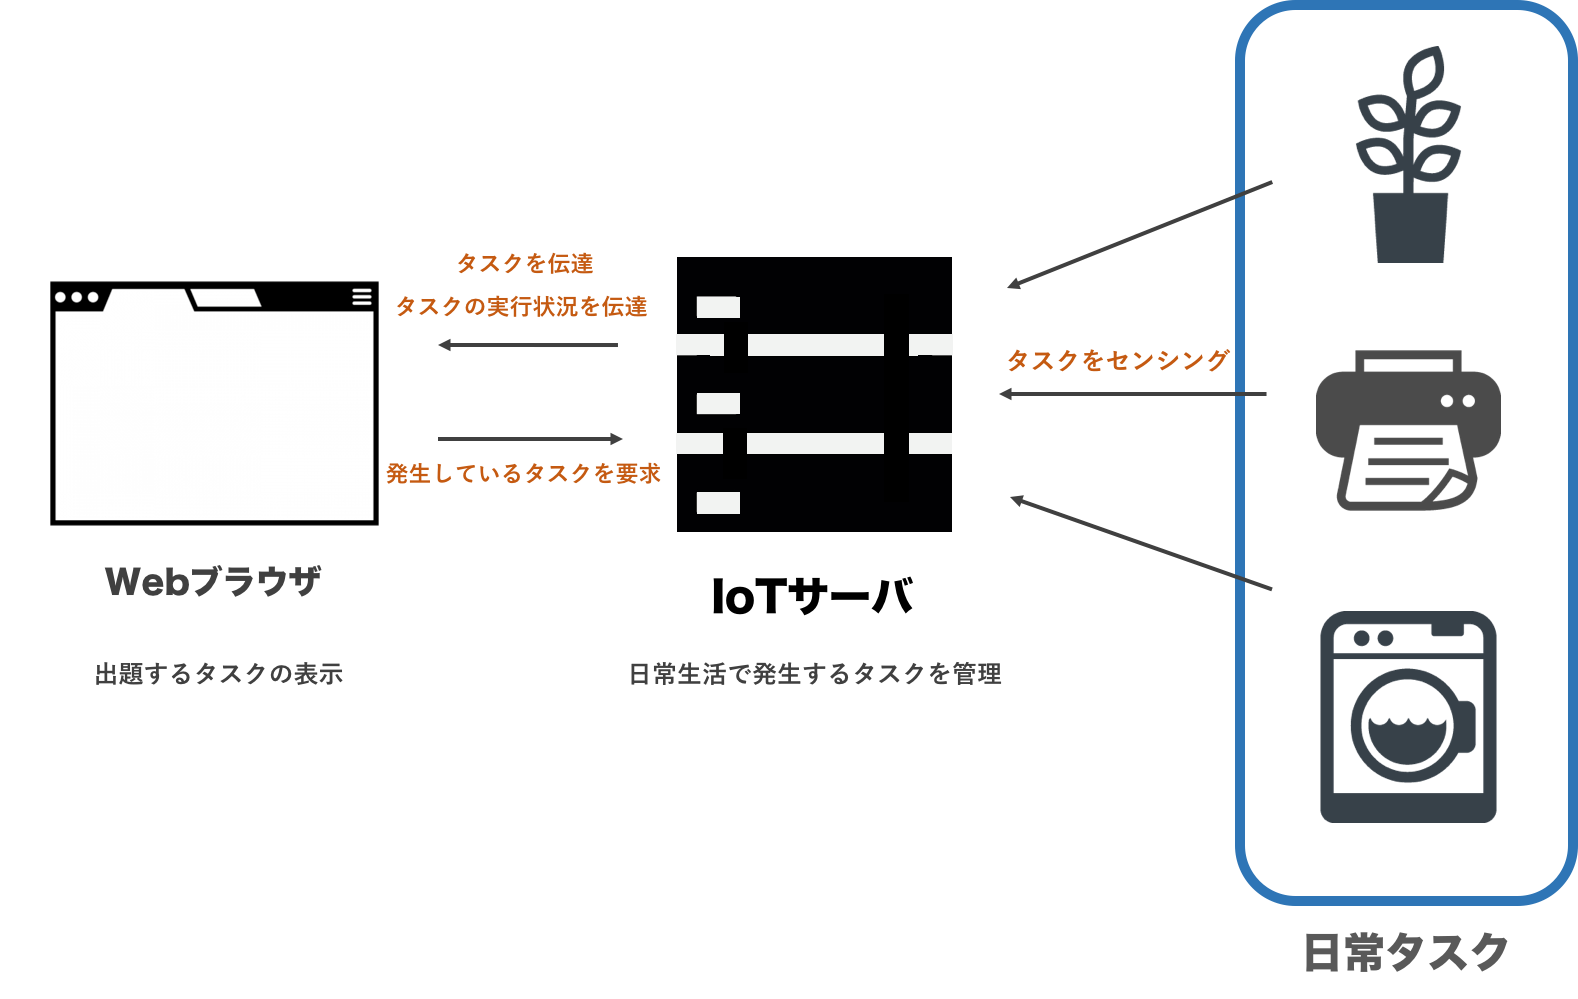
\includegraphics[width=\textwidth,height=5cm,keepaspectratio]{images/2493299280.png}
\caption{}
\label{fig:2493299280.png}\end{figure}

\section{実験}\label{ux5b9fux9a13}

\subsection{本システムがチューリングテストとして利用できるのかの検証}\label{ux672cux30b7ux30b9ux30c6ux30e0ux304cux30c1ux30e5ux30fcux30eaux30f3ux30b0ux30c6ux30b9ux30c8ux3068ux3057ux3066ux5229ux7528ux3067ux304dux308bux306eux304bux306eux691cux8a3c}

\subsubsection{実験手法}\label{ux5b9fux9a13ux624bux6cd5}

\subsubsection{結果}\label{ux7d50ux679c}

\subsubsection{考察}\label{ux8003ux5bdf}

\subsection{遂行を要求されるタスクの許容量の調査}\label{ux9042ux884cux3092ux8981ux6c42ux3055ux308cux308bux30bfux30b9ux30afux306eux8a31ux5bb9ux91cfux306eux8abfux67fb}

\subsubsection{実験手法}\label{ux5b9fux9a13ux624bux6cd5-1}

\subsubsection{結果}\label{ux7d50ux679c-1}

\subsubsection{考察}\label{ux8003ux5bdf-1}

\section{参考文献}\label{ux53c2ux8003ux6587ux732e}
